\documentclass[conference]{IEEEtran}
\IEEEoverridecommandlockouts
% The preceding line is only needed to identify funding in the first footnote. If that is unneeded, please comment it out.
%Template version as of 6/27/2024

\usepackage{cite}
\usepackage{float}
\usepackage{url}
\usepackage{amsmath,amssymb,amsfonts}
\usepackage{algorithmic}
\usepackage{graphicx}
\usepackage{textcomp}
\usepackage{xcolor}
\def\BibTeX{{\rm B\kern-.05em{\sc i\kern-.025em b}\kern-.08em
    T\kern-.1667em\lower.7ex\hbox{E}\kern-.125emX}}
\begin{document}

\title{Comparison of Machine Learning Models for Predicting Depression in Adults Using Behavioral Biomarkers\\
{\footnotesize \textsuperscript{*}Note: Sub-titles are not captured for https://ieeexplore.ieee.org  and
should not be used}
\thanks{Identify applicable funding agency here. If none, delete this.}
}
\author{
\IEEEauthorblockN{1\textsuperscript{st} Caiza}
\IEEEauthorblockA{\textit{Departamento de Ciencias de la} \\
\textit{Computación} \\
\textit{Universidad de las Fuerzas Armadas}\\
\textit{ESPE}\\
Sangolquí, Ecuador \\
cdcaiza5@espe.edu.ec}
\and
\IEEEauthorblockN{2\textsuperscript{nd} Frias}
\IEEEauthorblockA{\textit{Departamento de Ciencias de la} \\
\textit{Computación} \\
\textit{Universidad de las Fuerzas Armadas}\\
\textit{ESPE}\\
Sangolquí, Ecuador \\
pafrias@espe.edu.ec}
\and
\IEEEauthorblockN{3\textsuperscript{rd} Villarroel}
\IEEEauthorblockA{\textit{Departamento de Ciencias de la} \\
\textit{Computación} \\
\textit{Universidad de las Fuerzas Armadas}\\
\textit{ESPE}\\
Sangolquí, Ecuador \\
jjvillarroel1@espe.edu.ec}
}

\maketitle

\begin{abstract}
This document is a model and instructions for \LaTeX.
This and the IEEEtran.cls file define the components of your paper [title, text, heads, etc.]. *CRITICAL: Do Not Use Symbols, Special Characters, Footnotes, 
or Math in Paper Title or Abstract.
\end{abstract}

\begin{IEEEkeywords}
machine learning, depression, predictive modeling, digital biomarkers, BRFSS
\end{IEEEkeywords}

\section{Introduction}

Major depressive disorder represents one of the most critical public health challenges globally, profoundly affecting patients' quality of life and straining healthcare systems. Traditionally, clinical diagnosis and treatment selection have relied heavily on subjective psychiatric evaluations and a reactive, ``trial and error'' paradigm \cite{sokolov_decoding_2024, popescu_evaluating_2021}%[cite: 3]. 
As the global burden of mental health disorders grows, there is an urgent need to transition toward proactive, preventative, and personalized psychiatric care.

In recent years, Artificial Intelligence (AI) has emerged as a transformative tool in psychiatric research and decision-making \cite{chiang_systematic_2025}%[cite: 3]. 
Cutting-edge studies have successfully applied machine learning (ML) and deep learning algorithms to predict depression using complex clinical biomarkers. For instance, predictive models have been trained on high-dimensional gray-matter structures from brain magnetic resonance imaging (MRI) \cite{jiang_applying_2026}%[cite: 3], 
blood DNA methylation profiles \cite{sokolov_decoding_2024}%[cite: 3], 
and multimodal sensing networks that integrate audio, video, and text data \cite{zhang_multimodal_2024}%[cite: 3]. 
Furthermore, AI-powered Clinical Decision Support Systems (CDSS) have been developed to predict psychotherapy remission rates \cite{kannampallil_cross-trial_2022}%[cite: 3], 
demonstrating clinical feasibility and acceptability without negatively impacting the physician-patient relationship during real-world consultations \cite{popescu_evaluating_2021, tanguay-sela_evaluating_2022}%[cite: 3].

Despite these significant technological advances, a notable gap remains in the translational application of these predictive models to routine clinical practice \cite{chiang_systematic_2025}%[cite: 3]. 
Many state-of-the-art diagnostic algorithms depend on expensive, highly specialized, or invasive data sources (e.g., neuroimaging or genomics) that are not readily available in standard primary care or community settings. However, few studies have deeply explored the predictive power of highly accessible, self-reported community health data to proactively estimate depression risk. There remains an unresolved need to evaluate how everyday socio-demographic, economic, and behavioral variables can act as reliable ``digital biomarkers'' on a large population scale.

To address this knowledge gap, this study aims to estimate the risk of depression in adults through a comparative evaluation of robust machine learning classifiers, utilizing everyday health variables and associated risk factors. By transforming static epidemiological data into a dynamic predictive tool, this research seeks to identify which behavioral and psychosocial biomarkers exhibit the strongest predictive influence on depression. Ultimately, the contribution of this work lies in demonstrating the viability of using accessible, non-invasive community data to support early risk detection and personalized psychiatric interventions.

The remainder of this article is organized as follows: Section II details the methodology, including the dataset extraction, feature ranking, and the configuration of the machine learning algorithms. Section III presents the experimental results and performance metrics. Section IV provides a discussion of the clinical implications of the findings. Finally, Section V concludes the paper and outlines future research directions.

\section{Method}

\subsection{Study Approach and Design}
This article develops a predictive and comparative study based on a quantitative and descriptive approach. The primary goal of the research is to estimate the risk of depression in adults through a comparative evaluation of machine learning algorithms, identifying which socio-demographic and behavioral biomarkers exert the greatest predictive influence. A non-experimental, cross-sectional design is proposed, analyzing retrospective epidemiological databases to construct a clinical classification model \cite{sokolov_decoding_2024} %[cite: 3].

\subsection{Development Methodology}
For the execution of the project, the CRISP-DM (Cross-Industry Standard Process for Data Mining) methodology \cite{chapman2000crisp} %[cite: 3] 
was adopted. This framework was chosen due to its cyclical and industry-standard structure, which is ideal for the systematic development of predictive models in the healthcare domain. The analytical tools were based on the Python programming language, utilizing specialized libraries such as Pandas \cite{mckinney2010pandas} %[cite: 3] 
for tabular manipulation via \texttt{pyreadstat} %[cite: 1], 
and Scikit-learn \cite{scikit-learn} %[cite: 3] 
for algorithmic modeling.

\subsection{Data Source and Extraction Methodology}
The analyzed data originate from the \textit{Behavioral Risk Factor Surveillance System} (BRFSS, 2024 cycle) %[cite: 1], 
a large-scale epidemiological surveillance survey conducted by the Centers for Disease Control and Prevention (CDC) \cite{cdc2024brfss} %[cite: 3]. 
The original dataset contains $455{,}006$ records and $301$ individual variables representing a wide array of population health metrics %[cite: 1]. 

To ensure computational efficiency and focus on the most relevant information, data extraction was managed using the \texttt{pyreadstat} library, selectively loading only the required columns directly from the \texttt{.XPT} file %[cite: 1]. 
This extraction methodology prevents memory overload and speeds up the preprocessing pipeline %[cite: 1]. 
For the feature-selection step, a $100{,}000$-row subsample was used to keep the RF and mutual-information rankings tractable; the selected set was then evaluated on the full $455{,}006$-row dataset %[cite: 1].

\subsection{Study Variables and Target Definition}

The definitive clinical target variable for this predictive model is \texttt{ADDEPEV3}, which represents whether a patient has ever been told by a health professional that they have a depressive disorder \cite{cdc2024brfss} %[cite: 1, 2, 3]. 
During the data preparation pipeline, this categorical variable is binarized, mapping positive diagnoses to 1 and negative diagnoses to 0, while non-responses are discarded to maintain the integrity of the supervised learning process %[cite: 1]. 
While other depression-related variables exist in the dataset (e.g., \texttt{\_MENT14D}), \texttt{ADDEPEV3} was selected as the primary target due to its direct and definitive clinical diagnostic value %[cite: 1, 2].

Feature selection was performed by training a Random Forest classifier on the $100{,}000$-row subsample over the full $301$-column universe (excluding the $11$ variables listed in the supplementary material: \texttt{ADDEPEV3}, \texttt{\_STATE}, \texttt{SEQNO}, \texttt{\_PSU}, \texttt{\_STRWT}, \texttt{\_WT2RAKE}, \texttt{\_LLCPWT}, \texttt{\_LLCPWT2}, \texttt{\_CLLCPWT}, \texttt{IDATE}, \texttt{WEIGHT2}) and ranking variables by Gini importance. The canonical set is the top-$30$ by RF importance. Two documented substitutions were applied: \texttt{\_MENT14D} (rank 2 in RF) was excluded because it is a near-duplicate of the target \texttt{ADDEPEV3}, and \texttt{\_STSTR} (rank 30) was excluded because it is a sampling stratum rather than a predictor. \texttt{\_PACKYRS} (RF rank 36) and \texttt{MEDCOST1} (RF rank 47) were substituted in to replace them. The literal next 2 RF ranks ($31$ and $32$, importances $0.00605$ and $0.00572$) were not used: rank 31 is the mean-encoded form of \texttt{\_RACE} which is already represented outside the 30-count, and rank 32 (\texttt{\_CASTHM1}) is a redundant legacy variant of \texttt{\_ASTHMS1} at rank 17. The $100{,}000$-row subsample was used for the selector alone (Random Forest fitting, mutual information, and permutation importance are not tractable on $455{,}006$ rows for the full universe); the chosen predictor set was then trained and evaluated on the full $455{,}006$-row dataset for the $5$-fold cross-validation. The final preset \texttt{default} therefore contains $30$ raw predictors (8 numeric, 4 ordinal, 18 categorical), with \texttt{\_RACE} mean-encoded separately; the model therefore receives $31$ input features per row. The full RF ranking is provided in Appendix~\ref{app:rf} %[cite: 1].

As detailed in Table \ref{tab_rf_importance}, the chosen set spans cognitive and psychosocial states (\texttt{DECIDE}, \texttt{DIFFALON}, \texttt{SDLONELY}, \texttt{LSATISFY}), self-reported mental and physical health days (\texttt{MENTHLTH}, \texttt{POORHLTH}, \texttt{PHYSHLTH}, \texttt{\_PHYS14D}, \texttt{\_RFHLTH}, \texttt{GENHLTH}), demographic and anthropometric variables (\texttt{\_AGE80}, \texttt{\_AGEG5YR}, \texttt{\_SEX}, \texttt{SEXVAR}, \texttt{CELLSEX3}, \texttt{\_BMI5}, \texttt{HEIGHT3}, \texttt{WTKG3}), socioeconomic and behavioural indicators (\texttt{EMPLOY1}, \texttt{MEDCOST1}, \texttt{ECIGNOW3}, \texttt{\_PACKYRS}), and chronic-condition and screening history (\texttt{ASTHMA3}, \texttt{\_LTASTH1}, \texttt{\_ASTHMS1}, \texttt{HAVARTH4}, \texttt{\_DRDXAR2}, \texttt{HIVTST7}, \texttt{\_AIDTST4}, \texttt{HIVTSTD3}).

\begin{table}[htbp]
\caption{Top-30 Predictors of the Preset \texttt{default} (RF-ranked)}
\begin{center}
\scriptsize
\setlength{\tabcolsep}{3pt}
\renewcommand{\arraystretch}{1.15}
\begin{tabular}{|l|c|p{4.0cm}|}
\hline
\textbf{Variable} & \textbf{Type} & \textbf{Brief Description} \\
\hline
MENTHLTH   & numeric     & Number of days with poor mental health \\
POORHLTH   & numeric     & Days where poor health limited usual activities \\
DECIDE     & categorical & Difficulty concentrating, remembering, or making decisions \\
\_PHYS14D  & categorical & 14+ days of poor physical health \\
PHYSHLTH   & numeric     & Number of days with poor physical health \\
GENHLTH    & ordinal     & Self-reported general health \\
SDLONELY   & ordinal     & Frequency of feeling lonely / socially isolated \\
DIFFALON   & categorical & Difficulty doing errands alone \\
\_RFHLTH   & categorical & Self-reported good or better general health \\
\_SEX      & categorical & Biological sex \\
SEXVAR     & categorical & Sex variable \\
ECIGNOW3   & categorical & Current e-cigarette use \\
\_AGE80    & numeric     & Imputed age (top-coded at 80) \\
EMPLOY1    & categorical & Current employment status \\
ASTHMA3    & categorical & Ever diagnosed with asthma \\
\_ASTHMS1  & categorical & Computed current asthma status \\
\_AGEG5YR  & ordinal     & Age, 5-year bands \\
\_BMI5     & numeric     & Computed Body Mass Index \\
LSATISFY   & ordinal     & Self-reported life satisfaction \\
HIVTST7    & categorical & Ever tested for HIV \\
\_LTASTH1  & categorical & Computed lifetime asthma status \\
\_DRDXAR2  & categorical & Computed diagnosed arthritis status \\
CELLSEX3   & categorical & Sex variable from the cellular-phone sample \\
\_AIDTST4  & categorical & Computed indicator: ever been tested for HIV \\
HIVTSTD3   & categorical & Date / recency of last HIV test \\
HEIGHT3    & numeric     & Reported height \\
HAVARTH4   & categorical & Ever diagnosed with arthritis \\
WTKG3      & numeric     & Computed weight in kg \\
\_PACKYRS  & numeric     & Computed pack-years of smoking \\
MEDCOST1   & categorical & Could not see a doctor because of cost \\
\hline
\multicolumn{3}{|p{8cm}|}{\footnotesize Plus \texttt{\_RACE} (mean-encoded; encoded column at RF rank 31, importance 0.00605; see Section II.E).} \\
\hline
\multicolumn{3}{|p{8cm}|}{\footnotesize \textit{Note.} Variables are listed in RF-importance order on the 100k subsample. \texttt{\_MENT14D} (RF rank 2) and \texttt{\_STSTR} (RF rank 30) are excluded by documented substitution; \texttt{\_PACKYRS} and \texttt{MEDCOST1} substitute in. The full RF ranking is provided in Appendix~\ref{app:rf}.} \\
\hline
\end{tabular}
\label{tab_rf_importance}
\end{center}
\end{table}

\subsection{Data Preparation and Processing}
Data cleaning constituted a critical phase to avoid mathematical biases. According to the BRFSS codebook \cite{cdc2024brfss} %[cite: 3], 
specific numerical codes like $7$, $8$, $9$, $14$, $77$, $99$, and $9999$ represent non-responses (e.g., ``Don't know'' or ``Refused'') %[cite: 1]. 
These were mapped to \textit{NaN} to prevent models from interpreting them as continuous weights %[cite: 1]. 
Additionally, values of $88$ in \texttt{PHYSHLTH}, \texttt{MENTHLTH}, and \texttt{POORHLTH} (meaning ``None'') were explicitly mapped to $0$ to preserve their clinical meaning %[cite: 1].

Categorical variables were processed using smoothed mean encoding and One-Hot Encoding, while numerical variables were normalized using a Standard Scaler %[cite: 1]. 
The single \texttt{\_RACE} column is mean-encoded rather than one-hot-encoded: a single regularised numeric effect is easier to interpret in isolation and avoids one-hot encoding amplifying racial-disparity patterns in downstream predictions, while the smoothing prior ($\alpha=10$) prevents overfitting on small groups %[cite: 1]. 
Of the seven race-ethnicity variables available in BRFSS 2024 (\texttt{\_RACE}, \texttt{\_RACEGR3}, \texttt{\_RACEG21}, \texttt{\_RACEPRV}, \texttt{\_IMPRACE}, \texttt{\_MRACE1}, \texttt{\_CRACE1}), \texttt{\_RACE} was selected as the canonical CDC reporting standard; the other variables are alternative cardinalities or non-Hispanic-specific cuts of the same construct and would not change the model materially %[cite: 1]. 
Race was included as a feature for two reasons. Empirically, the encoded column has RF rank $31$ with Gini importance $0.00605$, placing it above all variables below the top-$30$ cutoff; the model is marginally better with it than without. Clinically, depression prevalence is known to vary systematically by race in US epidemiological data due to a combination of social determinants (discrimination, healthcare access) and measurement effects (underdiagnosis in some groups, overdiagnosis in others); the encoded form lets the model learn this baseline. We note that the inclusion of race in a depression-prediction model has known fairness implications and that the fairness properties of the model are not separately validated in this study; the choice is documented here so that downstream users can make an informed decision about deployment %[cite: 1]. 
Finally, missing values were imputed using the median for numeric/ordinal data and the mode for categorical data %[cite: 1].

\subsection{Dataset Partitioning and Balancing Justification}
Given the highly imbalanced nature of epidemiological datasets (where healthy individuals vastly outnumber those with depression), a $5$-fold Stratified Cross-Validation (\texttt{StratifiedKFold}) technique was implemented over the full $455{,}006$-row dataset %[cite: 1]. 
This methodology ensures that the exact proportion of the target class is preserved across all training and validation folds, allowing for robust evaluation %[cite: 1]. 

Class imbalance was addressed with \texttt{class\_weight="balanced"} across all five models. No resampling technique was applied. Synthetic resampling (SMOTENC) was also tried on a subsample and was discarded for the same reason: it did not improve any of the worst-case metrics and increased training time without changing the model ranking %[cite: 1].

\subsection{Data Modeling and Hyperparameter Justification}
Five machine learning architectures were deployed. The five models were configured with the hyperparameters shown in Table~\ref{tab:hyperparams}; all five used \texttt{class\_weight="balanced"} and \texttt{random\_state=42} for reproducibility. An additional hyperparameter-tuning loop was attempted on a subsample and was discarded because it produced no meaningful gain on F1 or PR-AUC and did not change the model ranking.

\begin{itemize}
    \item \textbf{Random Forest:} an ensemble of decision trees trained on bootstrapped samples with random feature subsets, aggregated by majority vote.
    \item \textbf{Linear SVC:} a linear support-vector classifier wrapped in \texttt{CalibratedClassifierCV} to expose probability estimates from the SVM margins.
    \item \textbf{Logistic Regression:} a linear model using a logistic link, with the \texttt{newton-cholesky} solver for efficient fitting on large dense data.
    \item \textbf{XGBoost:} a depth-wise gradient-boosting ensemble with regularized objective.
    \item \textbf{LightGBM:} a leaf-wise gradient-boosting ensemble optimized for high-dimensional, mixed-type data.
\end{itemize}

\subsection{Evaluation Metrics}
Instead of relying solely on baseline accuracy, the models were evaluated using a comprehensive suite of metrics appropriate for imbalanced clinical data, avoiding theoretical mathematical derivations in favor of applied clinical relevance:

\begin{itemize}
    \item \textbf{F1-Score \& Recall:} Recall (Sensitivity) measures the model's ability to identify true depression cases, minimizing dangerous false negatives. The F1-Score provides the harmonic mean between precision and recall, ensuring a balanced performance. %[cite: 1]
    \item \textbf{ROC-AUC \& PR-AUC:} The Area Under the Receiver Operating Characteristic (ROC-AUC) curve evaluates the model's discriminative threshold. Given the class imbalance, the Precision-Recall AUC (PR-AUC) was also calculated to provide a stricter performance penalty for false positives. %[cite: 1]
    \item \textbf{Brier Score \& Confusion Matrix:} The Brier score measures the exactness of the probabilistic outputs, while the accumulated Confusion Matrix provides a direct visualization of true positive, true negative, false positive, and false negative predictions across the $5$ folds. %[cite: 1]
\end{itemize}

In addition to the standard probability metrics, the per-model decision threshold was tuned out-of-fold by maximizing F1 (default); the \texttt{youden} (Youden's $J$) and \texttt{cost} (cost-sensitive with user-defined cost ratio) options are available for screening and cost-sensitive applications. The reported \texttt{*@thr} rows show metrics at the chosen threshold, and \texttt{threshold} reports the threshold itself. In this paper we report the F1-tuned threshold (5-fold mean). %[cite: 1]

\subsection{Implementation Environment}
The system was implemented using a high-performance computational environment executed via Python scripts. Mathematical processing relied on NumPy \cite{harris2020array} %[cite: 3] 
and Pandas \cite{mckinney2010pandas} %[cite: 3] 
modules, while the machine learning experimentation framework depended on the Scikit-Learn \cite{scikit-learn} %[cite: 3] 
ecosystem.


\section{Results}

The findings of the predictive modeling experiment are presented based on the evaluation of five machine learning architectures over a $5$-fold stratified cross-validation process on the full $455{,}006$-row dataset. The algorithms were evaluated on their ability to detect the \texttt{ADDEPEV3} target using the $30$ socio-behavioral biomarkers of the preset \texttt{default}. Thresholds are tuned per model out-of-fold to maximize F1; the \texttt{*@thr} columns report metrics at the chosen threshold, while the unsubscripted accuracy is reported at the $0.5$ default threshold.

Table \ref{tab:model_results} summarizes the performance metrics for each model. XGBoost achieves the highest unsubscripted accuracy ($0.840$) and the lowest Brier score ($0.116$), indicating the best-calibrated probability estimates. XGBoost and LightGBM are tied for the highest ROC-AUC ($0.843$) and PR-AUC ($0.635$). Under the F1-tuned threshold, XGBoost and LightGBM also tie for the highest F1 ($0.597$): LightGBM is marginally ahead in recall ($0.652$ vs $0.644$) and XGBoost is marginally ahead in precision ($0.556$ vs $0.552$). 

LinearSVC shows the largest swing from the $0.5$-threshold to the F1-tuned threshold: at $0.5$ it has the second-highest accuracy on the validation set ($0.833$, behind only XGBoost at $0.840$) but very low recall ($0.378$). F1-tuning moves the threshold down to $0.248$ and raises recall to $0.638$ at the cost of precision, giving F1 $0.577$. The linear baseline and the tree-based bagging model (Random Forest) reach similar F1 at the tuned threshold ($0.578$ and $0.581$ respectively) and lag the gradient-boosting pair on ROC-AUC, PR-AUC, and Brier. Appendix Table~\ref{tab:metrics_at_0.5} lists all five threshold-dependent metrics at the default $0.5$ threshold for direct comparison.

\begin{table}[htbp]
\caption{Model Evaluation Results (5-fold Mean, Full 455,006-row Dataset)}
\label{tab:model_results}
\centering
\scriptsize
\setlength{\tabcolsep}{3pt}
\renewcommand{\arraystretch}{1.15}
\resizebox{\columnwidth}{!}{
\begin{tabular}{|l|c|c|c|c|c|c|c|c|c|c|}
\hline
\textbf{Model} & \textbf{Acc@0.5} & \textbf{Acc@thr} & \textbf{Prec@thr} & \textbf{Rec@thr} & \textbf{F1@thr} & \textbf{Spec@thr} & \textbf{ROC-AUC} & \textbf{PR-AUC} & \textbf{Brier} & \textbf{Threshold} \\
\hline
Random Forest        & 0.769 & 0.803 & 0.528 & 0.646 & 0.581 & 0.845 & 0.831 & 0.612 & 0.171 & 0.553 \\
\hline
Linear SVC           & 0.833 & 0.802 & 0.526 & 0.638 & 0.577 & 0.846 & 0.825 & 0.607 & 0.121 & 0.248 \\
\hline
Logistic Regression  & 0.783 & 0.801 & 0.523 & 0.646 & 0.578 & 0.842 & 0.826 & 0.608 & 0.164 & 0.545 \\
\hline
XGBoost              & \textbf{0.840} & 0.816 & 0.556 & 0.644 & 0.597 & 0.862 & \textbf{0.843} & \textbf{0.635} & \textbf{0.116} & 0.304 \\
\hline
LightGBM             & 0.775 & 0.814 & 0.552 & 0.652 & 0.597 & 0.858 & \textbf{0.843} & 0.635 & 0.157 & 0.614 \\
\hline
\end{tabular}
}
\end{table}

\begin{table}[!t]
\caption{Model Hyperparameters}
\label{tab:hyperparams}
\centering
\scriptsize
\setlength{\tabcolsep}{3pt}
\renewcommand{\arraystretch}{1.15}
\begin{tabular}{|l|p{6.0cm}|}
\hline
\textbf{Model} & \textbf{Hyperparameters} \\
\hline
Random Forest       & \texttt{n\_estimators=300}, \texttt{max\_depth=12}, \texttt{n\_jobs=-1}, \texttt{random\_state=42}, \texttt{class\_weight="balanced"} \\
\hline
Linear SVC          & \texttt{LinearSVC(dual="auto", max\_iter=2000, class\_weight="balanced")} wrapped in \texttt{CalibratedClassifierCV(cv=3, method="sigmoid")} \\
\hline
Logistic Regression & \texttt{solver="newton-cholesky"}, \texttt{max\_iter=2000}, \texttt{random\_state=42}, \texttt{class\_weight="balanced"} \\
\hline
XGBoost             & \texttt{n\_estimators=300}, \texttt{max\_depth=6}, \texttt{learning\_rate=0.1}, \texttt{n\_jobs=-1}, \texttt{class\_weight="balanced"} \\
\hline
LightGBM            & \texttt{n\_estimators=300}, \texttt{learning\_rate=0.1}, \texttt{n\_jobs=-1}, \texttt{random\_state=42}, \texttt{class\_weight="balanced"} \\
\hline
\end{tabular}
\end{table}

The accumulated confusion matrices detail the specific classification behavior across the evaluated folds. As observed in Figure \ref{fig:cm_lightgbm}, LightGBM correctly identifies the largest share of true-positive depression cases at the F1-tuned threshold while keeping the false-negative count low. In contrast, while XGBoost (Figure \ref{fig:cm_xgboost}) reaches a comparable true-positive count, its higher threshold-driven precision is paired with a higher true-negative count, reflecting its advantage in calibration.

\begin{figure}[htbp]
\centering
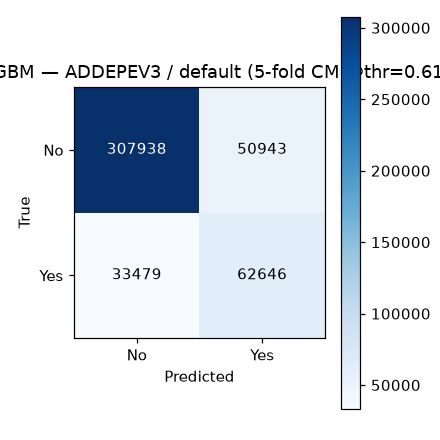
\includegraphics[width=0.35\textwidth]{Imagenes/cm_LightGBM_ADDEPEV3_default_class_weight.png}
\caption{Confusion Matrix for LightGBM (5-fold Cross-Validation, F1-Tuned Threshold)}
\label{fig:cm_lightgbm}
\end{figure}

\begin{figure}[htbp]
\centering
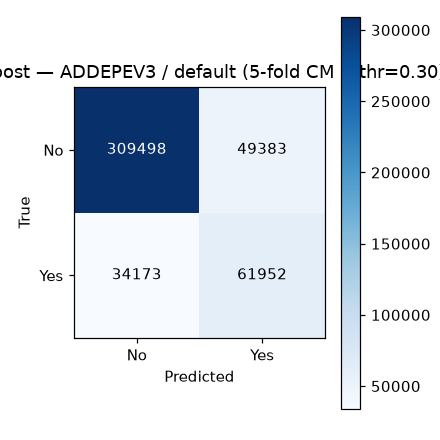
\includegraphics[width=0.35\textwidth]{Imagenes/cm_XGBoost_ADDEPEV3_default_class_weight.png}
\caption{Confusion Matrix for XGBoost (5-fold Cross-Validation, F1-Tuned Threshold)}
\label{fig:cm_xgboost}
\end{figure}

\section{Discussion}

The primary objective of this study was to estimate the risk of depression in adults by identifying the most influential socio-behavioral biomarkers and evaluating various predictive algorithms. The results indicate that gradient boosting frameworks—specifically LightGBM and XGBoost—are highly effective at modeling complex, non-linear epidemiological data, surpassing traditional linear approaches on both ranking and calibration metrics. 

A critical finding of this research is the importance of threshold choice when reporting results on imbalanced clinical data. Under a fixed $0.5$ threshold, the SVM and gradient-boosting models favour the majority class and miss a large share of positive cases (LinearSVC recall $0.378$, XGBoost recall $0.441$). F1-tuning the threshold per model closes this gap, with all five models reaching F1 $\in [0.577, 0.597]$ and recall $\in [0.638, 0.652]$. The remaining separation is in calibration: XGBoost and LightGBM share the top ROC-AUC ($0.843$) and PR-AUC ($0.635$), and XGBoost has the best Brier score ($0.116$), making it the strongest single candidate when well-calibrated probabilities are required. LightGBM reaches the same ROC-AUC with marginally higher recall ($0.652$ vs $0.644$) at the F1-tuned threshold, consistent with LightGBM's leaf-wise design for high-dimensional, mixed-type data. LinearSVC and Logistic Regression are competitive on F1 at the tuned threshold but trail on Brier and on PR-AUC.

Despite these promising results, the study presents methodological limitations. The reliance on the BRFSS dataset implies that the input variables are self-reported, making them susceptible to recall bias and subjective underreporting of symptoms. Furthermore, even after F1-tuning, the precision across all models remains moderate ($0.52$–$0.56$), reflecting an inherent challenge when working with highly imbalanced epidemiological data where symptoms overlap with other conditions.

Future research should focus on mitigating this residual false-positive rate through more advanced resampling or cost-sensitive learning. In addition, future work should evaluate the same predictors on a target measuring \textit{recent} depressive symptoms, in a setup where \texttt{\_MENT14D} is excluded from predictors to avoid target–predictor overlap. This would test transfer from lifetime-diagnosis to acute-risk prediction.

\section{Conclusions}

This study successfully demonstrated that machine learning algorithms can reliably estimate the risk of lifetime depression in adults utilizing accessible, non-invasive behavioral and psychosocial data. By identifying key digital biomarkers, this research confirms that everyday variables—such as socioeconomic status, mental and physical health self-reports, cognitive function, and behavioral indicators—hold substantial predictive power, reducing the reliance on costly clinical tests.

Among the evaluated architectures, XGBoost and LightGBM are tied at the top of the metric table. XGBoost is the strongest single model when well-calibrated probabilities are required (Brier $0.116$, ROC-AUC $0.843$, F1@thr $0.597$), while LightGBM reaches the same ROC-AUC with marginally higher recall ($0.652$ vs $0.644$) at the F1-tuned threshold.

The developed predictive framework offers direct practical applications for healthcare systems. These models can be seamlessly integrated into Clinical Decision Support Systems (CDSS) within primary care settings to automatically flag at-risk individuals using standard patient intake forms. Future investigations should expand the feature set and focus on longitudinal validations to further refine the precision of the algorithm in diverse clinical environments.

\appendix
\section{Feature selection evidence}

Table~\ref{app:rf} lists the Random Forest Gini-importance top-30 that produced the \texttt{default} preset, plus the two substituted-in variables from later RF ranks. Rows marked with a single asterisk are excluded from the preset; rows marked with a double asterisk are substituted in.

\begin{table}[H]
\caption{Random Forest Top-30 by Gini Importance (canonical)\,$^{\mathrm{a}}$}
\label{app:rf}
\centering
\scriptsize
\setlength{\tabcolsep}{3pt}
\renewcommand{\arraystretch}{1.1}
\begin{tabular}{|c|l|c|}
\hline
\textbf{Rank} & \textbf{Variable} & \textbf{Importance} \\
\hline
1  & MENTHLTH   & 0.15857 \\
2  & \_MENT14D$^{*}$  & 0.14782 \\
3  & POORHLTH   & 0.07117 \\
4  & DECIDE     & 0.05926 \\
5  & \_PHYS14D  & 0.02364 \\
6  & PHYSHLTH   & 0.02300 \\
7  & GENHLTH    & 0.01447 \\
8  & SDLONELY   & 0.01446 \\
9  & DIFFALON   & 0.01355 \\
10 & \_RFHLTH   & 0.01305 \\
11 & \_SEX      & 0.01217 \\
12 & SEXVAR     & 0.01164 \\
13 & ECIGNOW3   & 0.01133 \\
14 & \_AGE80    & 0.01007 \\
15 & EMPLOY1    & 0.00950 \\
16 & ASTHMA3    & 0.00900 \\
17 & \_ASTHMS1  & 0.00887 \\
18 & \_AGEG5YR  & 0.00877 \\
19 & \_BMI5     & 0.00876 \\
20 & LSATISFY   & 0.00815 \\
21 & HIVTST7    & 0.00791 \\
22 & \_LTASTH1  & 0.00717 \\
23 & \_DRDXAR2  & 0.00714 \\
24 & CELLSEX3   & 0.00712 \\
25 & \_AIDTST4  & 0.00676 \\
26 & HIVTSTD3   & 0.00667 \\
27 & HEIGHT3    & 0.00649 \\
28 & HAVARTH4   & 0.00638 \\
29 & WTKG3      & 0.00637 \\
30 & \_STSTR$^{*}$    & 0.00632 \\
36 & \_PACKYRS$^{**}$  & 0.00502 \\
47 & MEDCOST1$^{**}$   & 0.00380 \\
\hline
\multicolumn{3}{|p{8cm}|}{\footnotesize $^{\mathrm{a}}$\textit{Note.} $^{*}$Excluded from the preset by documented substitution: \texttt{\_MENT14D} (rank 2) as a near-duplicate of the target, \texttt{\_STSTR} (rank 30) as a sampling stratum. $^{**}$Substituted in from later RF ranks to replace the excluded rows: \texttt{\_PACKYRS} (rank 36), \texttt{MEDCOST1} (rank 47). The full ranking over all candidate variables is included in the supplementary material.} \\
\hline
\end{tabular}
\end{table}

\begin{table}[!t]
\caption{Model Performance at the Default $0.5$ Threshold (5-fold Mean, Full 455,006-row Dataset)}
\label{tab:metrics_at_0_5}
\centering
\scriptsize
\setlength{\tabcolsep}{4pt}
\renewcommand{\arraystretch}{1.15}
\begin{tabular}{|l|c|c|c|c|c|}
\hline
\textbf{Model} & \textbf{Acc@0.5} & \textbf{Prec@0.5} & \textbf{Rec@0.5} & \textbf{F1@0.5} & \textbf{Spec@0.5} \\
\hline
Random Forest       & 0.769 & 0.469 & 0.728 & 0.571 & 0.780 \\
\hline
Linear SVC          & \textbf{0.833} & \textbf{0.693} & 0.378 & 0.489 & \textbf{0.955} \\
\hline
Logistic Regression & 0.783 & 0.490 & 0.691 & 0.573 & 0.808 \\
\hline
XGBoost             & \textbf{0.840} & 0.691 & 0.441 & 0.538 & 0.947 \\
\hline
LightGBM            & 0.775 & 0.480 & \textbf{0.750} & \textbf{0.585} & 0.782 \\
\hline
\multicolumn{6}{|p{8cm}|}{\footnotesize \textit{Note.} All five metrics are evaluated at the default $0.5$ decision threshold (no per-model tuning). Compare against Table~\ref{tab:model_results} which reports the same metrics at the F1-tuned per-model threshold; the contrast illustrates the F1-vs-accuracy trade-off for imbalanced classification. Threshold-independent metrics (ROC-AUC, PR-AUC, Brier) are unchanged and are not repeated here.} \\
\hline
\end{tabular}
\end{table}

\bibliographystyle{ieeetr} 
\bibliography{Principal_Data} 

\vspace{12pt}
\end{document} 
